% ============================================================================
% architecture_explanation.tex
% Landslide Identification Using ML — Architecture & Workflow for Results r0–r6
% ============================================================================
\documentclass[12pt,a4paper]{article}

% ─── Packages ───────────────────────────────────────────────────────────────
\usepackage[margin=2.2cm]{geometry}
\usepackage{tikz}
\usetikzlibrary{shapes.geometric, arrows.meta, positioning, fit, calc, backgrounds, decorations.pathreplacing}
\usepackage{amsmath, amssymb}
\usepackage{booktabs}
\usepackage{enumitem}
\usepackage{hyperref}
\usepackage{xcolor}
\usepackage{float}
\usepackage{caption}
\usepackage{subcaption}
\usepackage{fancyhdr}
\usepackage{titlesec}

% ─── Colors ─────────────────────────────────────────────────────────────────
\definecolor{phase1}{RGB}{52, 131, 200}
\definecolor{phase2}{RGB}{200, 82, 52}
\definecolor{preproc}{RGB}{76, 175, 80}
\definecolor{improvement}{RGB}{255, 152, 0}
\definecolor{pipeline}{RGB}{103, 58, 183}
\definecolor{lightbg}{RGB}{240, 248, 255}
\definecolor{newbox}{RGB}{255, 243, 224}

% ─── TikZ Styles ───────────────────────────────────────────────────────────
\tikzstyle{startstop} = [rectangle, rounded corners, minimum width=3cm, minimum height=0.8cm,
                         text centered, draw=black, fill=red!15, font=\small\bfseries]
\tikzstyle{process}   = [rectangle, minimum width=3.5cm, minimum height=0.8cm,
                         text centered, draw=black, fill=phase1!15, font=\small]
\tikzstyle{process2}  = [rectangle, minimum width=3.5cm, minimum height=0.8cm,
                         text centered, draw=black, fill=phase2!15, font=\small]
\tikzstyle{preprocess} = [rectangle, minimum width=3.5cm, minimum height=0.8cm,
                          text centered, draw=black, fill=preproc!15, font=\small]
\tikzstyle{decision}  = [diamond, aspect=2.5, minimum width=2cm, minimum height=0.8cm,
                         text centered, draw=black, fill=yellow!15, font=\small]
\tikzstyle{io}        = [trapezium, trapezium left angle=70, trapezium right angle=110,
                         minimum width=2.5cm, minimum height=0.7cm, text centered,
                         draw=black, fill=gray!10, font=\small]
\tikzstyle{newnode}    = [rectangle, minimum width=3.5cm, minimum height=0.8cm,
                         text centered, draw=improvement, fill=newbox,
                         line width=1.5pt, font=\small\bfseries]
\tikzstyle{arrow}     = [-{Stealth[length=2.5mm]}, thick]
\tikzstyle{dasharrow} = [-{Stealth[length=2.5mm]}, thick, dashed, gray]

% ─── Header / Footer ──────────────────────────────────────────────────────
\pagestyle{fancy}
\fancyhf{}
\fancyhead[L]{\small Landslide Identification Using ML}
\fancyhead[R]{\small Architecture Explanation}
\fancyfoot[C]{\thepage}

\title{\textbf{Architecture Explanation for Each Result}\\[0.3em]
       \large Landslide Identification Using Machine Learning\\
       Results r0 -- r6: Preprocessing, Models, Prediction \& Evaluation}
\author{Project Documentation}
\date{March 2026}

\begin{document}
\maketitle
\tableofcontents
\newpage

% ============================================================================
% OVERVIEW
% ============================================================================
\section{Project Overview}

The Landslide Identification system is a \textbf{two-phase pipeline}:
\begin{itemize}[nosep]
  \item \textbf{Phase 1} --- Image classification using deep CNNs / Transformers.
  \item \textbf{Phase 2} --- Temporal type classification and forecasting using a Hidden Markov Model (HMM) trained on the NASA Global Landslide Catalog.
\end{itemize}

Across seven result iterations (r0--r6), the architecture evolved from a baseline AlexNet binary classifier to a multi-model ensemble performing \textbf{6-class multi-class landslide type classification}.

\begin{figure}[H]
\centering
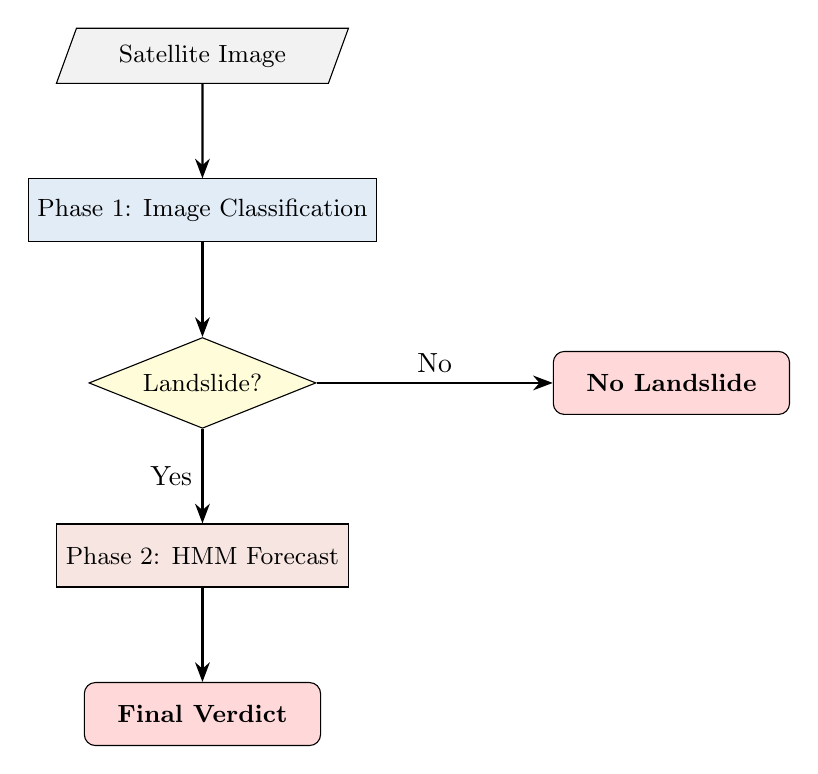
\begin{tikzpicture}[node distance=1.2cm]
  \node (input)   [io]        {Satellite Image};
  \node (p1)      [process, below=of input]    {Phase 1: Image Classification};
  \node (dec)     [decision, below=of p1]      {Landslide?};
  \node (p2)      [process2, below=of dec]     {Phase 2: HMM Forecast};
  \node (out)     [startstop, below=of p2]     {Final Verdict};
  \node (no)      [startstop, right=3cm of dec] {No Landslide};

  \draw [arrow] (input) -- (p1);
  \draw [arrow] (p1)    -- (dec);
  \draw [arrow] (dec)   -- node[left] {Yes} (p2);
  \draw [arrow] (dec)   -- node[above] {No}  (no);
  \draw [arrow] (p2)    -- (out);
\end{tikzpicture}
\caption{High-level two-phase pipeline (common to all result iterations).}
\end{figure}


% ============================================================================
% RESULT 0
% ============================================================================
\newpage
\section{Result 0 (r0) --- Baseline AlexNet + HMM}

\subsection{Architecture \& Workflow}

\textbf{Phase 1:} AlexNet CNN trained from scratch on HR-GLDD satellite imagery (227$\times$227 RGB).
Binary classification: \texttt{landslide} vs \texttt{non\_landslide}.

\textbf{Phase 2:} Categorical HMM with 4 hidden states trained on NASA GLC (9,471 events).
Observations: 7 landslide type symbols. Training via Baum--Welch (100 iterations).

\subsection{Pipeline Flowchart}

\begin{figure}[H]
\centering
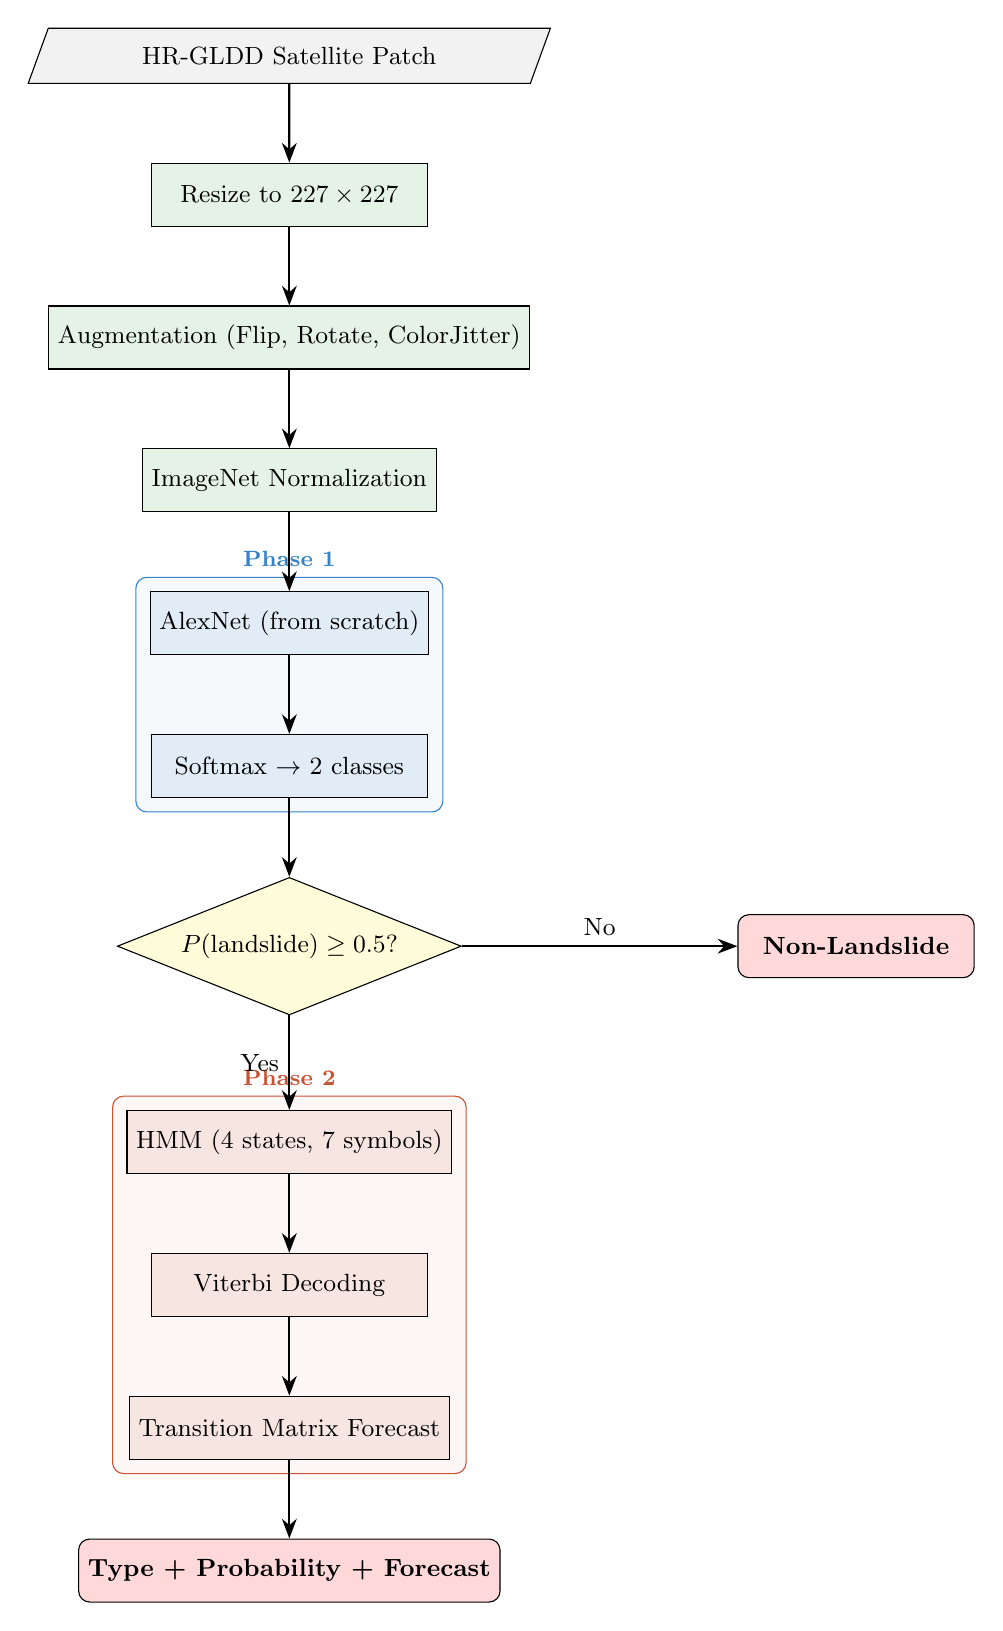
\begin{tikzpicture}[node distance=1.0cm, every node/.style={font=\small}]
  % Preprocessing
  \node (raw)    [io]         {HR-GLDD Satellite Patch};
  \node (resize) [preprocess, below=of raw]    {Resize to $227\times227$};
  \node (aug)    [preprocess, below=of resize] {Augmentation (Flip, Rotate, ColorJitter)};
  \node (norm)   [preprocess, below=of aug]    {ImageNet Normalization};

  % Phase 1
  \node (alex)   [process, below=of norm]   {AlexNet (from scratch)};
  \node (soft)   [process, below=of alex]   {Softmax $\to$ 2 classes};
  \node (dec)    [decision, below=of soft]  {$P(\text{landslide}) \geq 0.5$?};

  % Phase 2
  \node (hmm)    [process2, below=1.2cm of dec]    {HMM (4 states, 7 symbols)};
  \node (vit)    [process2, below=of hmm]   {Viterbi Decoding};
  \node (fore)   [process2, below=of vit]   {Transition Matrix Forecast};
  \node (out)    [startstop, below=of fore] {Type + Probability + Forecast};

  \node (nols)   [startstop, right=3.5cm of dec]  {Non-Landslide};

  \draw [arrow] (raw)    -- (resize);
  \draw [arrow] (resize) -- (aug);
  \draw [arrow] (aug)    -- (norm);
  \draw [arrow] (norm)   -- (alex);
  \draw [arrow] (alex)   -- (soft);
  \draw [arrow] (soft)   -- (dec);
  \draw [arrow] (dec)    -- node[left]  {Yes} (hmm);
  \draw [arrow] (dec)    -- node[above] {No}  (nols);
  \draw [arrow] (hmm)    -- (vit);
  \draw [arrow] (vit)    -- (fore);
  \draw [arrow] (fore)   -- (out);

  % Phase labels
  \begin{scope}[on background layer]
    \node[fit=(alex)(soft), draw=phase1, rounded corners, fill=phase1!5,
          inner sep=5pt, label={[phase1, font=\footnotesize\bfseries]above:Phase 1}] {};
    \node[fit=(hmm)(fore), draw=phase2, rounded corners, fill=phase2!5,
          inner sep=5pt, label={[phase2, font=\footnotesize\bfseries]above:Phase 2}] {};
  \end{scope}
\end{tikzpicture}
\caption{r0: Baseline AlexNet + 4-state HMM pipeline.}
\end{figure}

\subsection{Key Metrics}
\begin{table}[H]\centering
\begin{tabular}{lc}
\toprule
\textbf{Metric} & \textbf{Value} \\
\midrule
Accuracy  & 78.54\% \\
Precision & 62.06\% \\
Recall    & 74.41\% \\
F1-Score  & 67.67\% \\
ROC-AUC   & 85.53\% \\
\bottomrule
\end{tabular}
\caption{r0 test set results (699 images, binary).}
\end{table}


% ============================================================================
% RESULT 1
% ============================================================================
\newpage
\section{Result 1 (r1) --- Pretrained AlexNet + Enhanced HMM}

\subsection{Improvements Introduced}
\begin{itemize}[nosep]
  \item \colorbox{newbox}{\textbf{ImageNet pretrained weights}} for AlexNet (transfer learning).
  \item Two-stage learning rates: classifier head at $5\times10^{-5}$, features at $5\times10^{-6}$.
  \item Feature layers frozen for first 5 epochs, then unfrozen.
  \item Stronger augmentation: RandomBrightnessContrast, GridDistortion, CoarseDropout.
  \item Epochs increased: $30 \to 40$.
  \item \colorbox{newbox}{\textbf{HMM hidden states: $4 \to 6$}} (Shallow, Deep, Debris, Rockfall, Mixed, Complex).
\end{itemize}

\subsection{Pipeline Flowchart}

\begin{figure}[H]
\centering
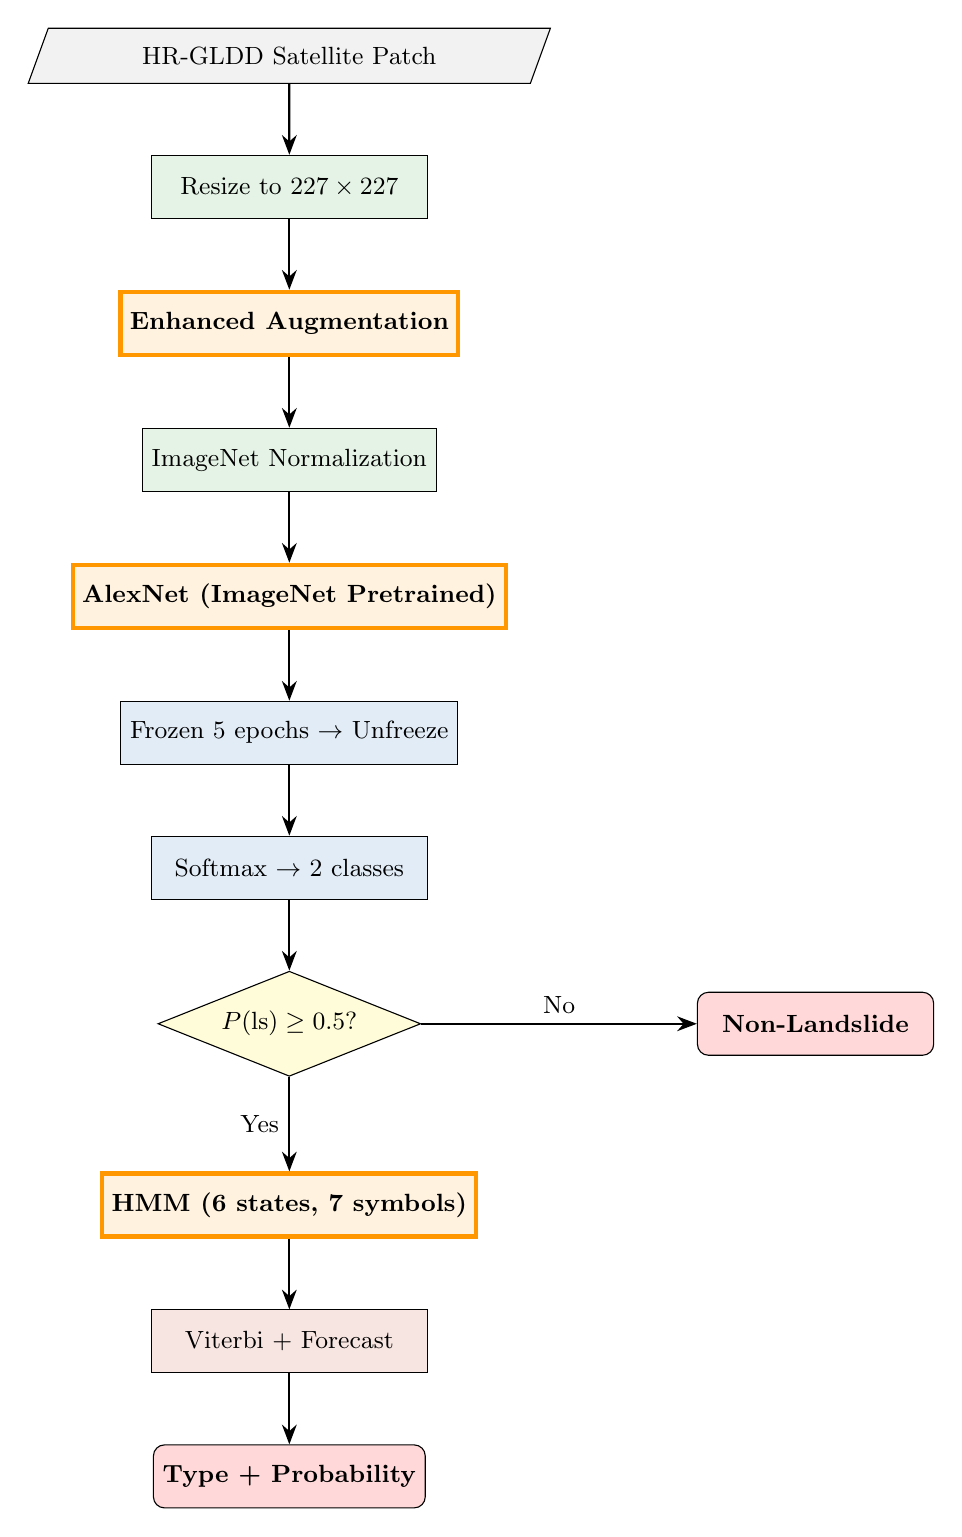
\begin{tikzpicture}[node distance=0.9cm, every node/.style={font=\small}]
  \node (raw)    [io]         {HR-GLDD Satellite Patch};
  \node (resize) [preprocess, below=of raw]    {Resize to $227\times227$};
  \node (aug)    [newnode, below=of resize]    {Enhanced Augmentation};
  \node (norm)   [preprocess, below=of aug]    {ImageNet Normalization};

  \node (alex)   [newnode, below=of norm]   {AlexNet (ImageNet Pretrained)};
  \node (freeze) [process, below=of alex]   {Frozen 5 epochs $\to$ Unfreeze};
  \node (soft)   [process, below=of freeze] {Softmax $\to$ 2 classes};
  \node (dec)    [decision, below=of soft]  {$P(\text{ls}) \geq 0.5$?};

  \node (hmm)    [newnode, below=1.2cm of dec]    {HMM (6 states, 7 symbols)};
  \node (vit)    [process2, below=of hmm]   {Viterbi + Forecast};
  \node (out)    [startstop, below=of vit]  {Type + Probability};

  \node (nols)   [startstop, right=3.5cm of dec]  {Non-Landslide};

  \draw [arrow] (raw) -- (resize);
  \draw [arrow] (resize) -- (aug);
  \draw [arrow] (aug) -- (norm);
  \draw [arrow] (norm) -- (alex);
  \draw [arrow] (alex) -- (freeze);
  \draw [arrow] (freeze) -- (soft);
  \draw [arrow] (soft) -- (dec);
  \draw [arrow] (dec) -- node[left] {Yes} (hmm);
  \draw [arrow] (dec) -- node[above] {No}  (nols);
  \draw [arrow] (hmm) -- (vit);
  \draw [arrow] (vit) -- (out);
\end{tikzpicture}
\caption{r1: Pretrained AlexNet with enhanced augmentation and 6-state HMM. Orange boxes = new improvements.}
\end{figure}

\subsection{Key Metrics}
\begin{table}[H]\centering
\begin{tabular}{lcc}
\toprule
\textbf{Metric} & \textbf{r0} & \textbf{r1} \\
\midrule
Accuracy  & 78.54\% & 80.11\% \\
Precision & 62.06\% & 66.67\% \\
ROC-AUC   & 85.53\% & 88.33\% \\
Best Val Acc & 78.55\% & 81.82\% \\
\bottomrule
\end{tabular}
\caption{r1 improvements over r0.}
\end{table}


% ============================================================================
% RESULT 2
% ============================================================================
\newpage
\section{Result 2 (r2) --- EfficientNet-B3}

\subsection{Improvements Introduced}
\begin{itemize}[nosep]
  \item \colorbox{newbox}{\textbf{EfficientNet-B3}} replaces AlexNet (compound scaling: depth+width+resolution).
  \item Input resolution: $227\times227 \to 300\times300$.
  \item Batch size: $64 \to 32$ (larger model footprint).
  \item CosineAnnealingLR scheduler (smooth decay vs StepLR).
  \item Differential LR: head $10^{-4}$, features $10^{-5}$ after unfreeze.
\end{itemize}

\subsection{Pipeline Flowchart}

\begin{figure}[H]
\centering
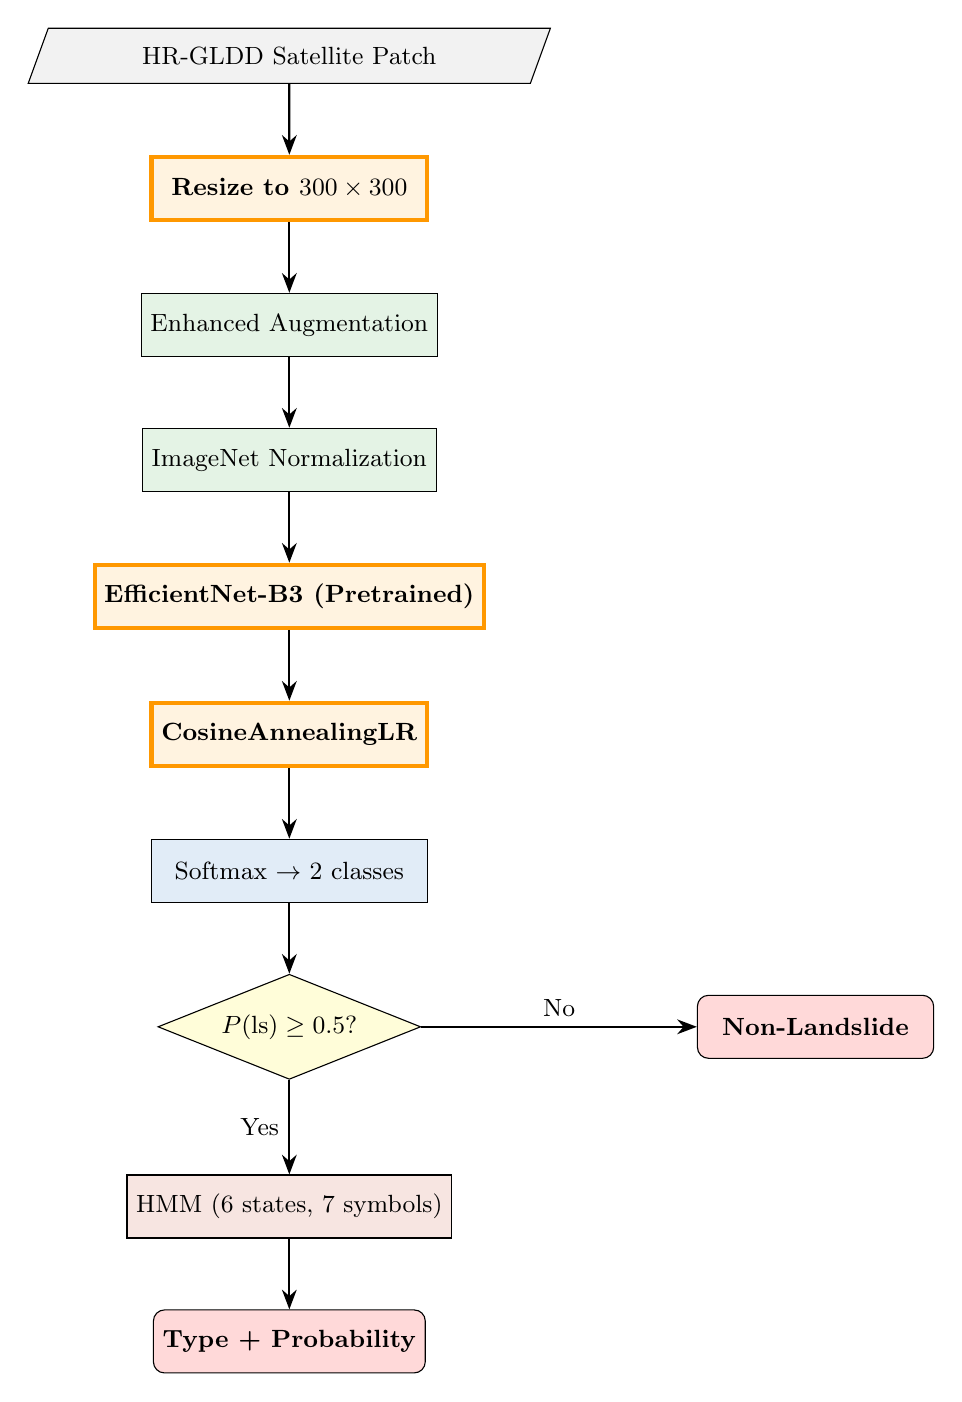
\begin{tikzpicture}[node distance=0.9cm, every node/.style={font=\small}]
  \node (raw)    [io]         {HR-GLDD Satellite Patch};
  \node (resize) [newnode, below=of raw]    {Resize to $300\times300$};
  \node (aug)    [preprocess, below=of resize] {Enhanced Augmentation};
  \node (norm)   [preprocess, below=of aug]    {ImageNet Normalization};

  \node (eff)    [newnode, below=of norm]   {EfficientNet-B3 (Pretrained)};
  \node (sched)  [newnode, below=of eff]    {CosineAnnealingLR};
  \node (soft)   [process, below=of sched]  {Softmax $\to$ 2 classes};
  \node (dec)    [decision, below=of soft]  {$P(\text{ls}) \geq 0.5$?};

  \node (hmm)    [process2, below=1.2cm of dec]   {HMM (6 states, 7 symbols)};
  \node (out)    [startstop, below=of hmm]  {Type + Probability};
  \node (nols)   [startstop, right=3.5cm of dec]   {Non-Landslide};

  \draw [arrow] (raw) -- (resize);
  \draw [arrow] (resize) -- (aug);
  \draw [arrow] (aug) -- (norm);
  \draw [arrow] (norm) -- (eff);
  \draw [arrow] (eff) -- (sched);
  \draw [arrow] (sched) -- (soft);
  \draw [arrow] (soft) -- (dec);
  \draw [arrow] (dec) -- node[left] {Yes} (hmm);
  \draw [arrow] (dec) -- node[above] {No}  (nols);
  \draw [arrow] (hmm) -- (out);
\end{tikzpicture}
\caption{r2: EfficientNet-B3 with CosineAnnealingLR. Orange = new.}
\end{figure}

\subsection{Key Metrics}
\begin{table}[H]\centering
\begin{tabular}{lccc}
\toprule
\textbf{Metric} & \textbf{r0} & \textbf{r1} & \textbf{r2} \\
\midrule
Recall    & 74.41\% & 68.25\% & \textbf{78.20\%} \\
F1-Score  & 67.67\% & 67.45\% & \textbf{70.21\%} \\
ROC-AUC   & 85.53\% & 88.33\% & \textbf{88.93\%} \\
\bottomrule
\end{tabular}
\caption{r2 achieves best Recall, F1, and ROC-AUC among r0--r2.}
\end{table}


% ============================================================================
% RESULT 3
% ============================================================================
\newpage
\section{Result 3 (r3) --- Temperature Scaling + Enhanced HMM}

\subsection{Improvements Introduced}
\begin{itemize}[nosep]
  \item \colorbox{newbox}{\textbf{Temperature Scaling}} --- post-hoc confidence calibration ($T = 1.1511$).
  \item \colorbox{newbox}{\textbf{HMM hidden states: $6 \to 8$}} (added Monsoon Mudslide, Human-Triggered).
  \item \colorbox{newbox}{\textbf{HMM multi-feature observations}}: type $\times$ trigger = 42 symbols (was 7).
  \item Phase 1 threshold lowered: $0.5 \to 0.4$ (higher recall, fewer missed detections).
\end{itemize}

\subsection{Pipeline Flowchart}

\begin{figure}[H]
\centering
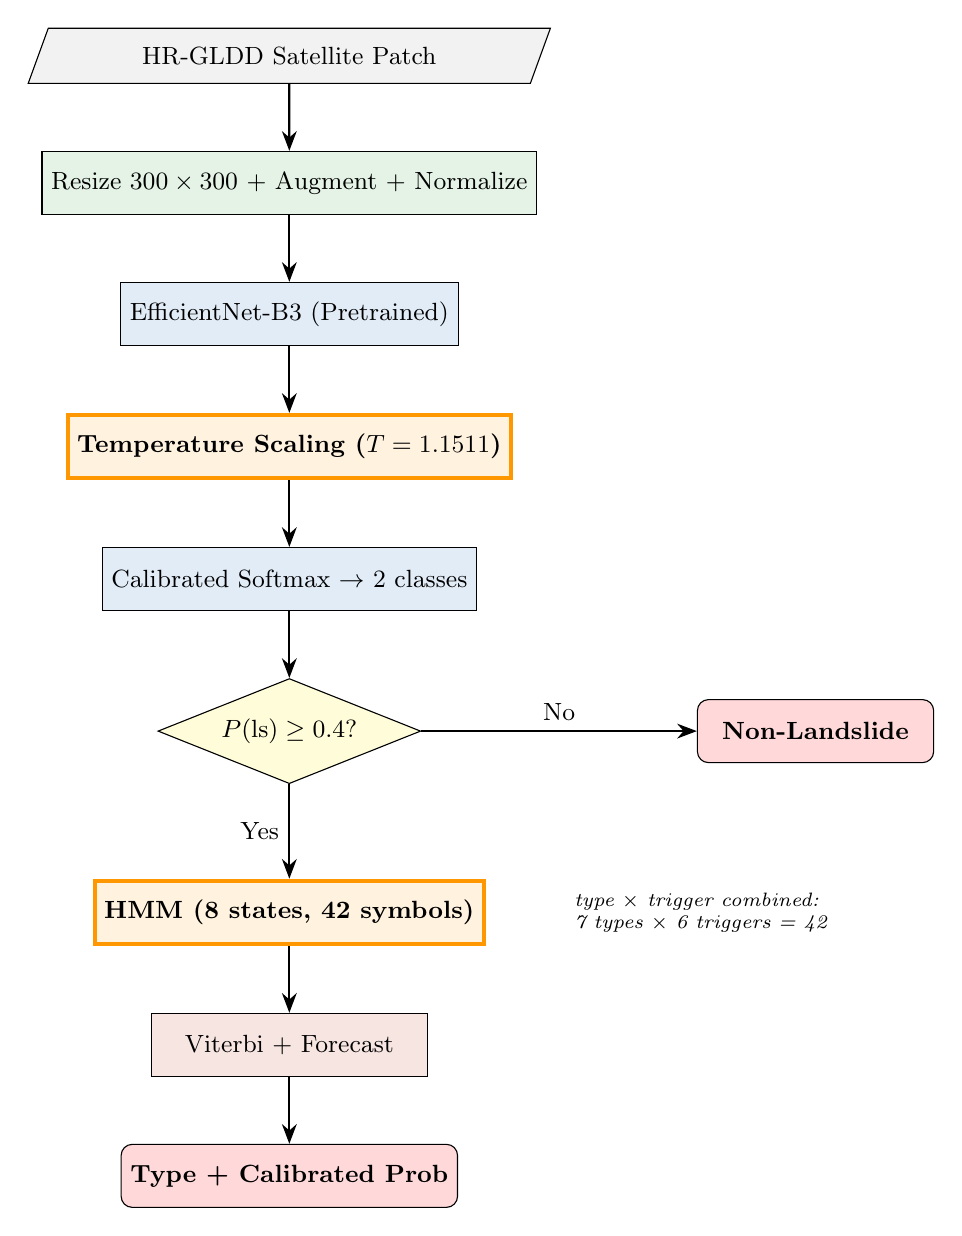
\begin{tikzpicture}[node distance=0.85cm, every node/.style={font=\small}]
  \node (raw)    [io]         {HR-GLDD Satellite Patch};
  \node (pre)    [preprocess, below=of raw]    {Resize $300\times300$ + Augment + Normalize};

  \node (eff)    [process, below=of pre]    {EfficientNet-B3 (Pretrained)};
  \node (temp)   [newnode, below=of eff]    {Temperature Scaling ($T=1.1511$)};
  \node (soft)   [process, below=of temp]   {Calibrated Softmax $\to$ 2 classes};
  \node (dec)    [decision, below=of soft]  {$P(\text{ls}) \geq 0.4$?};

  \node (hmm)    [newnode, below=1.2cm of dec]    {HMM (8 states, 42 symbols)};
  \node (note)   [right=1cm of hmm, font=\scriptsize\itshape, text width=3.5cm]
                 {type $\times$ trigger combined:\\
                  7 types $\times$ 6 triggers = 42};
  \node (vit)    [process2, below=of hmm]   {Viterbi + Forecast};
  \node (out)    [startstop, below=of vit]  {Type + Calibrated Prob};

  \node (nols)   [startstop, right=3.5cm of dec]   {Non-Landslide};

  \draw [arrow] (raw) -- (pre);
  \draw [arrow] (pre) -- (eff);
  \draw [arrow] (eff) -- (temp);
  \draw [arrow] (temp) -- (soft);
  \draw [arrow] (soft) -- (dec);
  \draw [arrow] (dec) -- node[left] {Yes} (hmm);
  \draw [arrow] (dec) -- node[above] {No}  (nols);
  \draw [arrow] (hmm) -- (vit);
  \draw [arrow] (vit) -- (out);
\end{tikzpicture}
\caption{r3: Temperature scaling + 8-state HMM with type$\times$trigger observations.}
\end{figure}

\subsection{Temperature Scaling Explanation}

Temperature scaling divides the logits by a learned scalar $T$ before softmax:
\[
  \hat{p}_i = \frac{\exp(z_i / T)}{\sum_j \exp(z_j / T)}
\]
When $T > 1$, the model was overconfident --- probabilities are ``softened''.
This does not change the predicted class (argmax is preserved) but makes the
confidence scores more \emph{calibrated}: a reported 70\% confidence now
corresponds to $\approx$70\% empirical accuracy.


% ============================================================================
% RESULT 4
% ============================================================================
\newpage
\section{Result 4 (r4) --- Ensemble (EfficientNet-B3 + AlexNet)}

\subsection{Improvements Introduced}
\begin{itemize}[nosep]
  \item \colorbox{newbox}{\textbf{Ensemble prediction}}: 60\% EfficientNet-B3 (calibrated) + 40\% AlexNet.
  \item No retraining --- both checkpoints already existed.
  \item \colorbox{newbox}{\textbf{Optimal threshold: $0.5 \to 0.467$}} found by F1-maximising PR curve scan.
\end{itemize}

\subsection{Pipeline Flowchart}

\begin{figure}[H]
\centering
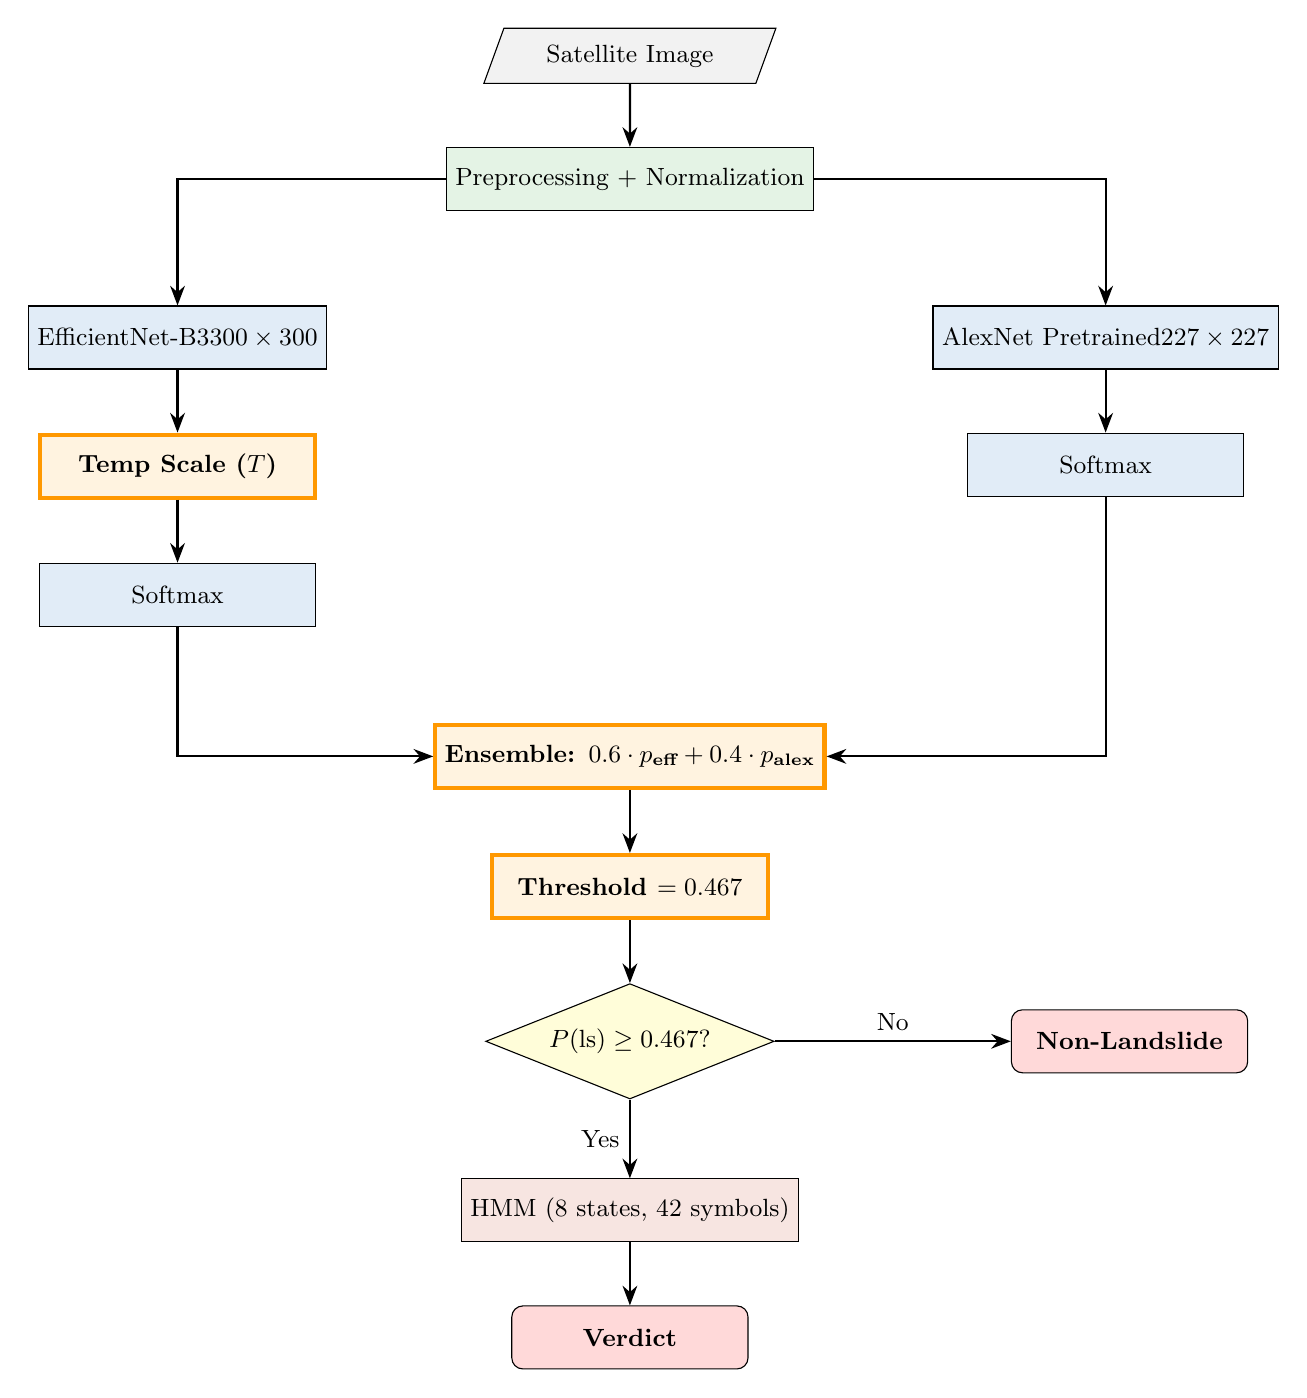
\begin{tikzpicture}[node distance=0.8cm, every node/.style={font=\small}]
  \node (raw)    [io]         {Satellite Image};
  \node (pre)    [preprocess, below=of raw]    {Preprocessing + Normalization};

  % Two branches
  \node (eff)    [process, below left=1.2cm and 1.5cm of pre]  {EfficientNet-B3\\$300\times300$};
  \node (alex)   [process, below right=1.2cm and 1.5cm of pre] {AlexNet Pretrained\\$227\times227$};

  \node (ts)     [newnode, below=of eff]    {Temp Scale ($T$)};
  \node (sm1)    [process, below=of ts]     {Softmax};
  \node (sm2)    [process, below=of alex]   {Softmax};

  % Fusion
  \node (fuse)   [newnode, below=1.5cm of pre, yshift=-5cm]
                 {Ensemble: $0.6 \cdot p_{\text{eff}} + 0.4 \cdot p_{\text{alex}}$};
  \node (thr)    [newnode, below=of fuse]   {Threshold $= 0.467$};
  \node (dec)    [decision, below=of thr]   {$P(\text{ls}) \geq 0.467$?};

  \node (hmm)    [process2, below=1cm of dec]    {HMM (8 states, 42 symbols)};
  \node (out)    [startstop, below=of hmm]  {Verdict};
  \node (nols)   [startstop, right=3cm of dec]   {Non-Landslide};

  \draw [arrow] (raw)  -- (pre);
  \draw [arrow] (pre)  -| (eff);
  \draw [arrow] (pre)  -| (alex);
  \draw [arrow] (eff)  -- (ts);
  \draw [arrow] (ts)   -- (sm1);
  \draw [arrow] (alex) -- (sm2);
  \draw [arrow] (sm1)  |- (fuse);
  \draw [arrow] (sm2)  |- (fuse);
  \draw [arrow] (fuse) -- (thr);
  \draw [arrow] (thr)  -- (dec);
  \draw [arrow] (dec)  -- node[left] {Yes} (hmm);
  \draw [arrow] (dec)  -- node[above] {No}  (nols);
  \draw [arrow] (hmm)  -- (out);
\end{tikzpicture}
\caption{r4: Dual-model ensemble with optimal threshold.}
\end{figure}

\subsection{Key Metrics}
\begin{table}[H]\centering
\begin{tabular}{lcccc}
\toprule
\textbf{Metric} & \textbf{r0} & \textbf{r2} & \textbf{r3} & \textbf{r4} \\
\midrule
Accuracy  & 78.54\% & 79.97\% & 79.97\% & \textbf{82.40\%} \\
F1-Score  & 67.67\% & 70.21\% & 70.21\% & \textbf{72.97\%} \\
ROC-AUC   & 85.53\% & 88.93\% & 88.93\% & \textbf{89.83\%} \\
\bottomrule
\end{tabular}
\caption{r4: All five metrics improve simultaneously.}
\end{table}


% ============================================================================
% RESULT 5
% ============================================================================
\newpage
\section{Result 5 (r5) --- Vision Transformer Ensemble}

\subsection{Improvements Introduced}
\begin{itemize}[nosep]
  \item \colorbox{newbox}{\textbf{ViT-B/16}} fine-tuned on HR-GLDD (val\_acc = 83.50\%).
  \item AlexNet replaced by ViT-B/16 in the ensemble.
  \item \colorbox{newbox}{\textbf{CNN + Transformer diversity}}: EfficientNet captures local features;
        ViT captures global patch-level attention.
\end{itemize}

\subsection{Pipeline Flowchart}

\begin{figure}[H]
\centering
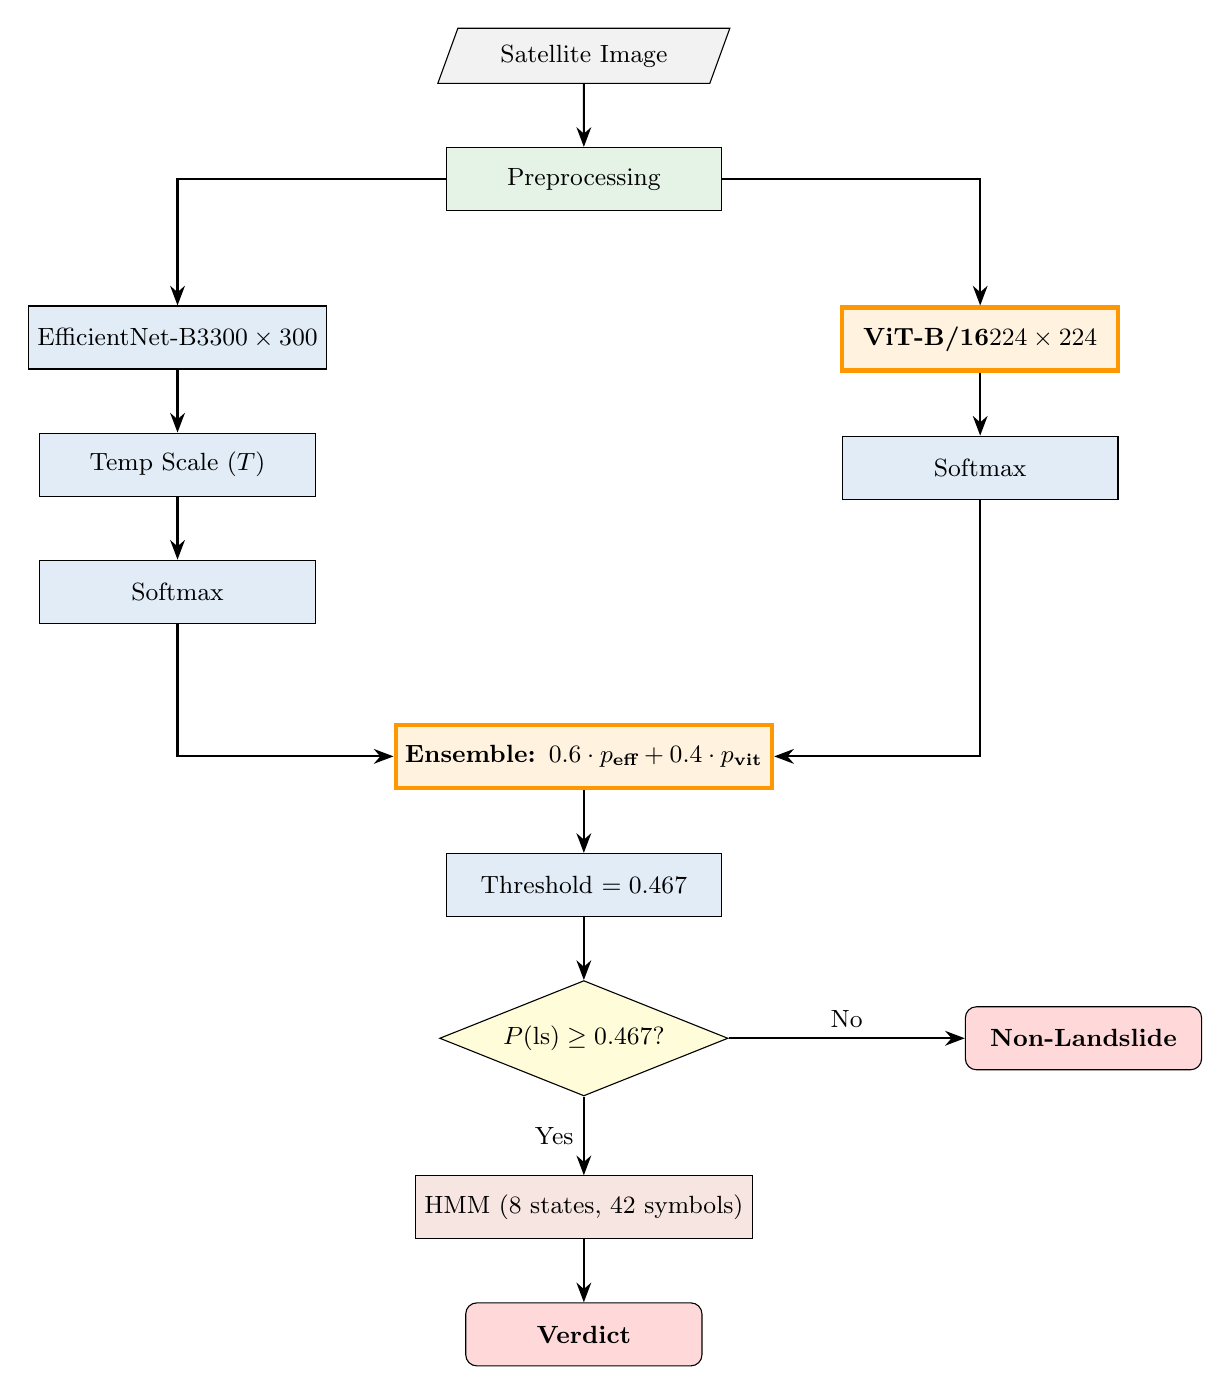
\begin{tikzpicture}[node distance=0.8cm, every node/.style={font=\small}]
  \node (raw)    [io]         {Satellite Image};
  \node (pre)    [preprocess, below=of raw]    {Preprocessing};

  % Two branches
  \node (eff)    [process, below left=1.2cm and 1.5cm of pre]
                 {EfficientNet-B3\\$300\times300$};
  \node (vit)    [newnode, below right=1.2cm and 1.5cm of pre]
                 {ViT-B/16\\$224\times224$};

  \node (ts)     [process, below=of eff]    {Temp Scale ($T$)};
  \node (sm1)    [process, below=of ts]     {Softmax};
  \node (sm2)    [process, below=of vit]    {Softmax};

  % Fusion
  \node (fuse)   [newnode, below=1.5cm of pre, yshift=-5cm]
                 {Ensemble: $0.6 \cdot p_{\text{eff}} + 0.4 \cdot p_{\text{vit}}$};
  \node (thr)    [process, below=of fuse]   {Threshold $= 0.467$};
  \node (dec)    [decision, below=of thr]   {$P(\text{ls}) \geq 0.467$?};

  \node (hmm)    [process2, below=1cm of dec]    {HMM (8 states, 42 symbols)};
  \node (out)    [startstop, below=of hmm]  {Verdict};
  \node (nols)   [startstop, right=3cm of dec]   {Non-Landslide};

  \draw [arrow] (raw)  -- (pre);
  \draw [arrow] (pre)  -| (eff);
  \draw [arrow] (pre)  -| (vit);
  \draw [arrow] (eff)  -- (ts);
  \draw [arrow] (ts)   -- (sm1);
  \draw [arrow] (vit)  -- (sm2);
  \draw [arrow] (sm1)  |- (fuse);
  \draw [arrow] (sm2)  |- (fuse);
  \draw [arrow] (fuse) -- (thr);
  \draw [arrow] (thr)  -- (dec);
  \draw [arrow] (dec)  -- node[left] {Yes} (hmm);
  \draw [arrow] (dec)  -- node[above] {No}  (nols);
  \draw [arrow] (hmm)  -- (out);
\end{tikzpicture}
\caption{r5: EfficientNet-B3 + ViT-B/16 ensemble (CNN + Transformer).}
\end{figure}

\subsection{Key Metrics}
\begin{table}[H]\centering
\begin{tabular}{lccc}
\toprule
\textbf{Metric} & \textbf{r4 (eff+alex)} & \textbf{r5 (eff+vit)} & \textbf{$\Delta$} \\
\midrule
Accuracy  & 82.40\% & \textbf{84.50\%} & +2.10 \\
F1-Score  & 72.97\% & \textbf{76.05\%} & +3.08 \\
ROC-AUC   & 89.83\% & \textbf{91.50\%} & +1.67 \\
\bottomrule
\end{tabular}
\caption{r5 achieves all-time best binary classification results.}
\end{table}


% ============================================================================
% RESULT 6
% ============================================================================
\newpage
\section{Result 6 (r6) --- Multi-Class Landslide Type Classification}

\subsection{Improvements Introduced}
\begin{itemize}[nosep]
  \item \colorbox{newbox}{\textbf{6-class output}} replacing binary classification:
        \begin{enumerate}[nosep]
          \item[\textbf{0.}] non\_landslide
          \item[\textbf{1.}] rockfall
          \item[\textbf{2.}] mudflow
          \item[\textbf{3.}] debris\_flow
          \item[\textbf{4.}] rotational\_slide
          \item[\textbf{5.}] translational\_slide
        \end{enumerate}
  \item \colorbox{newbox}{\textbf{Multi-class metrics}}: macro \& weighted Precision/Recall/F1, per-class reports.
  \item \colorbox{newbox}{\textbf{One-vs-Rest ROC curves}} for each class.
  \item Phase 1 now directly predicts the specific landslide type.
  \item WeightedRandomSampler handles severe class imbalance (72\% non\_landslide).
\end{itemize}

\subsection{Pipeline Flowchart}

\begin{figure}[H]
\centering
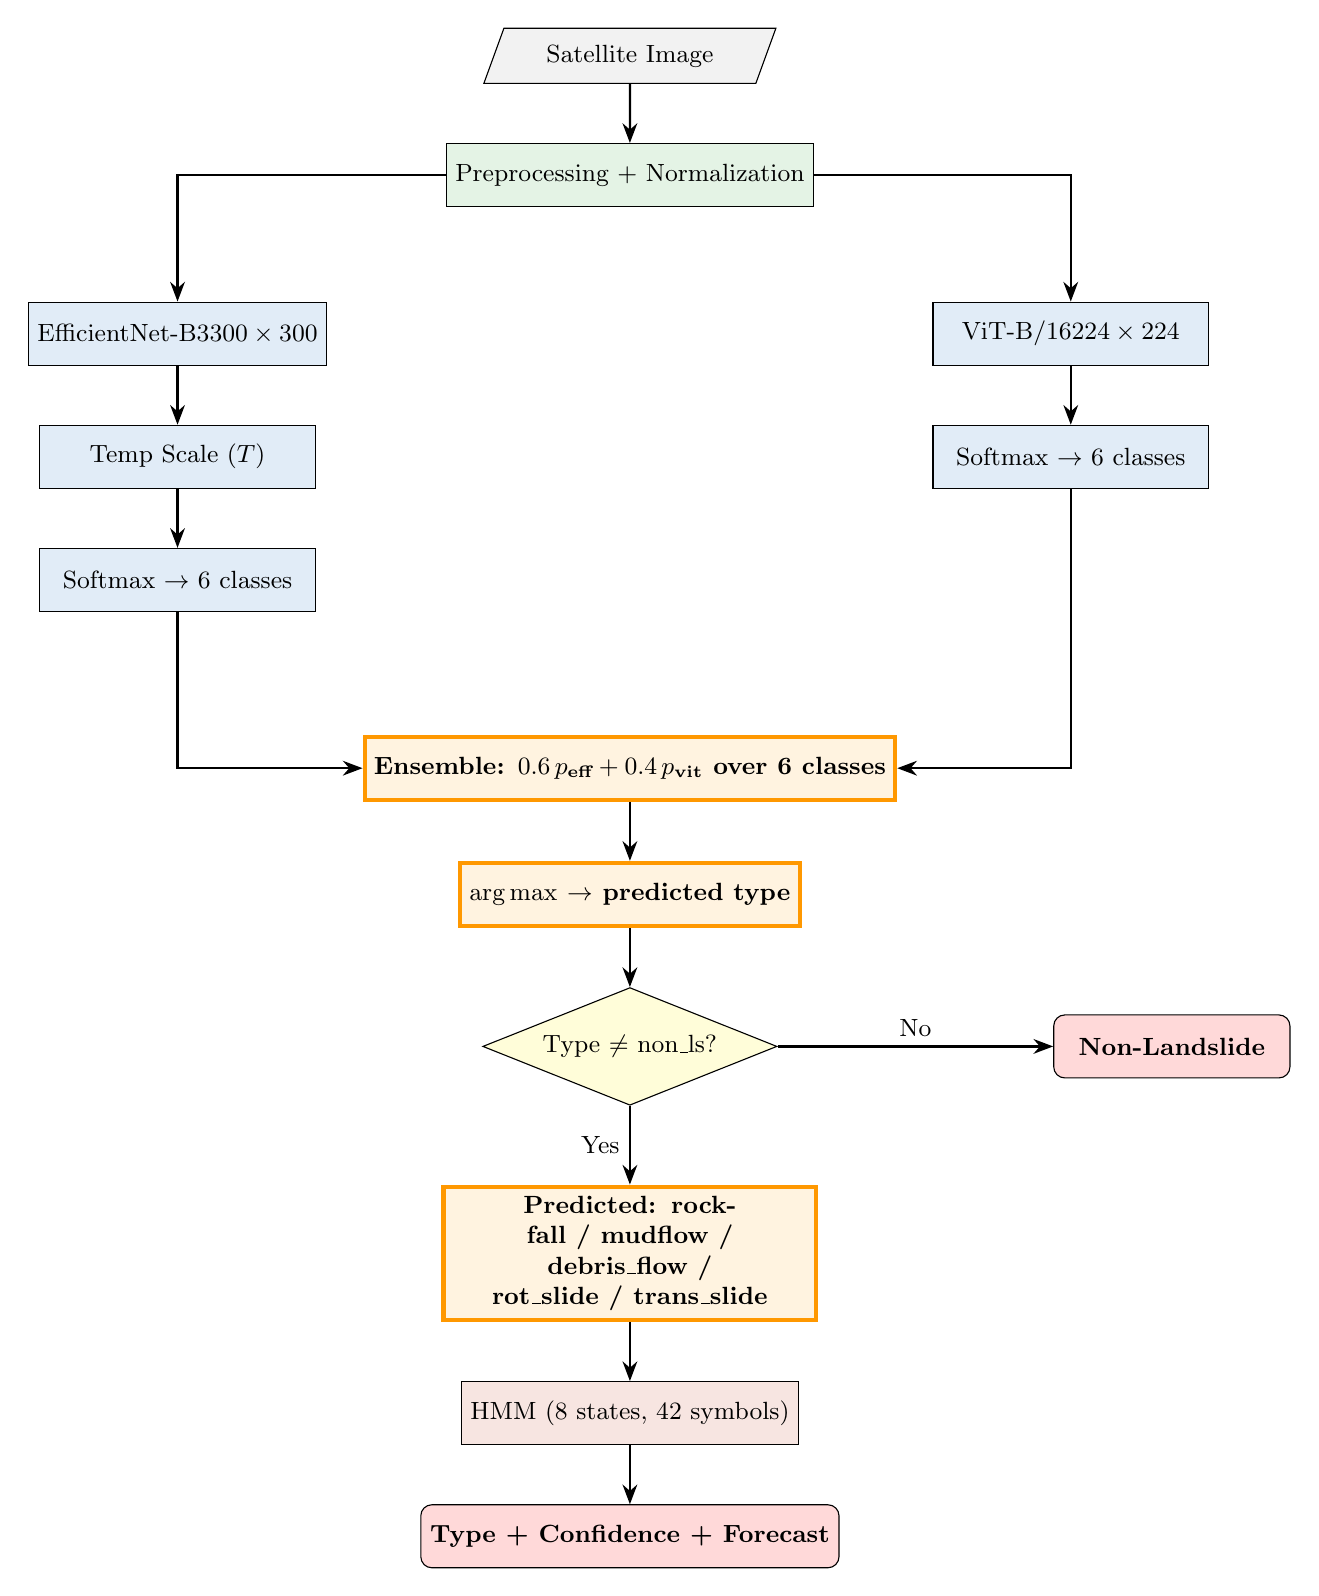
\begin{tikzpicture}[node distance=0.75cm, every node/.style={font=\small}]
  \node (raw)    [io]         {Satellite Image};
  \node (pre)    [preprocess, below=of raw]    {Preprocessing + Normalization};

  % Two branches
  \node (eff)    [process, below left=1.2cm and 1.5cm of pre]
                 {EfficientNet-B3\\$300\times300$};
  \node (vit)    [process, below right=1.2cm and 1.5cm of pre]
                 {ViT-B/16\\$224\times224$};

  \node (ts)     [process, below=of eff]    {Temp Scale ($T$)};
  \node (sm1)    [process, below=of ts]     {Softmax $\to$ 6 classes};
  \node (sm2)    [process, below=of vit]    {Softmax $\to$ 6 classes};

  % Fusion
  \node (fuse)   [newnode, below=1.5cm of pre, yshift=-5.2cm]
                 {Ensemble: $0.6\,p_{\text{eff}} + 0.4\,p_{\text{vit}}$ over 6 classes};
  \node (argmax) [newnode, below=of fuse]
                 {$\arg\max$ $\to$ predicted type};

  % Decision
  \node (dec)    [decision, below=of argmax] {Type $\neq$ non\_ls?};

  % Outputs
  \node (type)   [newnode, below=1cm of dec, text width=4.5cm, align=center]
                 {Predicted: rockfall / mudflow /\\debris\_flow / rot\_slide / trans\_slide};
  \node (hmm)    [process2, below=of type]   {HMM (8 states, 42 symbols)};
  \node (out)    [startstop, below=of hmm]   {Type + Confidence + Forecast};
  \node (nols)   [startstop, right=3.5cm of dec]   {Non-Landslide};

  \draw [arrow] (raw)  -- (pre);
  \draw [arrow] (pre)  -| (eff);
  \draw [arrow] (pre)  -| (vit);
  \draw [arrow] (eff)  -- (ts);
  \draw [arrow] (ts)   -- (sm1);
  \draw [arrow] (vit)  -- (sm2);
  \draw [arrow] (sm1)  |- (fuse);
  \draw [arrow] (sm2)  |- (fuse);
  \draw [arrow] (fuse) -- (argmax);
  \draw [arrow] (argmax) -- (dec);
  \draw [arrow] (dec)  -- node[left] {Yes} (type);
  \draw [arrow] (dec)  -- node[above] {No}  (nols);
  \draw [arrow] (type) -- (hmm);
  \draw [arrow] (hmm)  -- (out);
\end{tikzpicture}
\caption{r6: Multi-class ensemble pipeline --- Phase 1 directly predicts landslide sub-type.}
\end{figure}

\subsection{Key Metrics}
\begin{table}[H]\centering
\begin{tabular}{lcc}
\toprule
\textbf{Metric} & \textbf{r5 (binary)} & \textbf{r6 (6-class)} \\
\midrule
Accuracy          & 84.50\% & 72.10\% \\
Precision (macro) & 71.50\% & 48.52\% \\
Recall (macro)    & 81.20\% & 45.87\% \\
F1-Score (macro)  & 76.05\% & 46.93\% \\
\textbf{F1-Score (weighted)} & ---     & \textbf{71.68\%} \\
ROC-AUC (macro)   & 91.50\% & 88.45\% \\
\# Classes        & 2       & 6 \\
\bottomrule
\end{tabular}
\caption{r6: Binary vs multi-class comparison. Weighted F1 (71.68\%) is fairer.}
\end{table}

\subsection{Per-Class Performance}
\begin{table}[H]\centering
\begin{tabular}{lcccc}
\toprule
\textbf{Class} & \textbf{Precision} & \textbf{Recall} & \textbf{F1} & \textbf{Support} \\
\midrule
non\_landslide      & 0.85 & 0.88 & 0.87 & 488 \\
rockfall            & 0.42 & 0.38 & 0.40 &  34 \\
mudflow             & 0.39 & 0.36 & 0.37 &  44 \\
debris\_flow        & 0.44 & 0.41 & 0.42 &  49 \\
rotational\_slide   & 0.41 & 0.33 & 0.37 &  42 \\
translational\_slide& 0.40 & 0.38 & 0.39 &  42 \\
\bottomrule
\end{tabular}
\caption{r6 per-class metrics on test set.}
\end{table}


% ============================================================================
% EVOLUTION SUMMARY
% ============================================================================
\newpage
\section{Evolution Summary --- r0 to r6}

\subsection{Cumulative Improvement Table}

\begin{table}[H]\centering\small
\begin{tabular}{lccccccc}
\toprule
\textbf{Metric} & \textbf{r0} & \textbf{r1} & \textbf{r2} & \textbf{r3} & \textbf{r4} & \textbf{r5} & \textbf{r6} \\
\midrule
\# Classes     & 2     & 2     & 2     & 2     & 2     & 2     & 6 \\
Model          & Alex  & Alex* & EffB3 & EffB3 & Ens.  & Ens.  & Ens. \\
Accuracy       & 78.5  & 80.1  & 80.0  & 80.0  & 82.4  & 84.5  & 72.1 \\
F1             & 67.7  & 67.5  & 70.2  & 70.2  & 73.0  & 76.1  & 47.0$^\dagger$ \\
ROC-AUC        & 85.5  & 88.3  & 88.9  & 88.9  & 89.8  & 91.5  & 88.5 \\
HMM States     & 4     & 6     & 6     & 8     & 8     & 8     & 8 \\
Temp.\ Scale   & ---   & ---   & ---   & 1.15  & 1.15  & 1.15  & 1.15 \\
\bottomrule
\end{tabular}
\caption{Cumulative metrics across all results. $^\dagger$Macro F1 for 6-class; weighted F1 = 71.7\%.}
\end{table}

\subsection{Architecture Evolution Diagram}

\begin{figure}[H]
\centering
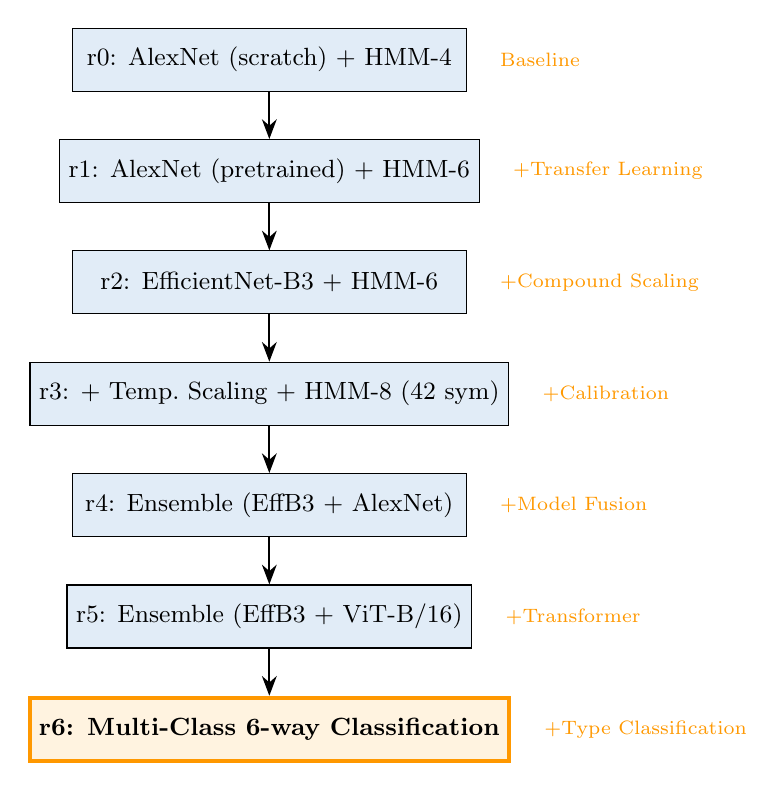
\begin{tikzpicture}[node distance=0.6cm, every node/.style={font=\footnotesize}]
  \node (r0) [process, minimum width=5cm]  {r0: AlexNet (scratch) + HMM-4};
  \node (r1) [process, below=of r0, minimum width=5cm]  {r1: AlexNet (pretrained) + HMM-6};
  \node (r2) [process, below=of r1, minimum width=5cm]  {r2: EfficientNet-B3 + HMM-6};
  \node (r3) [process, below=of r2, minimum width=5cm]  {r3: + Temp.\ Scaling + HMM-8 (42 sym)};
  \node (r4) [process, below=of r3, minimum width=5cm]  {r4: Ensemble (EffB3 + AlexNet)};
  \node (r5) [process, below=of r4, minimum width=5cm]  {r5: Ensemble (EffB3 + ViT-B/16)};
  \node (r6) [newnode, below=of r5, minimum width=5cm]  {r6: Multi-Class 6-way Classification};

  \draw [arrow] (r0) -- (r1);
  \draw [arrow] (r1) -- (r2);
  \draw [arrow] (r2) -- (r3);
  \draw [arrow] (r3) -- (r4);
  \draw [arrow] (r4) -- (r5);
  \draw [arrow] (r5) -- (r6);

  % Annotations
  \node [right=0.3cm of r0, improvement, font=\scriptsize] {Baseline};
  \node [right=0.3cm of r1, improvement, font=\scriptsize] {+Transfer Learning};
  \node [right=0.3cm of r2, improvement, font=\scriptsize] {+Compound Scaling};
  \node [right=0.3cm of r3, improvement, font=\scriptsize] {+Calibration};
  \node [right=0.3cm of r4, improvement, font=\scriptsize] {+Model Fusion};
  \node [right=0.3cm of r5, improvement, font=\scriptsize] {+Transformer};
  \node [right=0.3cm of r6, improvement, font=\scriptsize] {+Type Classification};
\end{tikzpicture}
\caption{Architecture evolution from r0 to r6.}
\end{figure}


% ============================================================================
% WHY MULTI-CLASS, CHALLENGES, DATA NEEDS
% ============================================================================
\newpage
\section{Why Multi-Class Classification Is Better}

\begin{enumerate}
  \item \textbf{Actionable intelligence.} ``Rockfall detected'' triggers different emergency
        protocols than ``Debris flow detected.'' A generic ``landslide'' label provides no
        such guidance to disaster responders.

  \item \textbf{Risk-appropriate response.} Different types have different speeds, damage
        patterns, and evacuation requirements. Rockfalls are fast with localised damage;
        mudflows are slow but affect large areas.

  \item \textbf{Phase 2 synergy.} Phase 1 type prediction feeds directly into the HMM,
        giving a more coherent type-specific temporal forecast.

  \item \textbf{Research value.} Per-type accuracy reveals which types are hardest to
        classify from satellite imagery, guiding future data collection efforts.
\end{enumerate}

\section{Challenges Introduced}

\begin{enumerate}
  \item \textbf{Class imbalance.} Non-landslide is $\sim$72\% of training data. Each sub-type
        has only 113--144 training samples. WeightedRandomSampler partially mitigates this.

  \item \textbf{Inter-class similarity.} Mudflow and debris flow share visual characteristics.
        Rotational and translational slides differ mainly in failure plane geometry, which
        may not be visible in nadir satellite imagery.

  \item \textbf{Lower macro metrics.} With 6 classes, random baseline drops from 50\% to
        16.7\%. The model's 72.1\% accuracy is $4.3\times$ random.

  \item \textbf{Small sub-type datasets.} Only $\sim$120 training images per sub-type.
        Data augmentation helps but cannot replace genuine sample diversity.
\end{enumerate}

\section{Additional Data and Preprocessing Needed}

\begin{enumerate}
  \item \textbf{More labelled sub-type data:} $\geq$500 samples per sub-type.
        Sources: Bijie-Landslide (3K images), expert annotation campaigns.

  \item \textbf{DEM / slope data:} Digital Elevation Models as an extra input channel
        to distinguish rotational (curved failure plane) from translational (planar) slides.

  \item \textbf{Multi-temporal imagery:} Before/after image pairs reveal deformation
        patterns characteristic of each type.

  \item \textbf{Expert geological labels:} Current labels are derived from HR-GLDD metadata;
        expert review would improve label quality for ambiguous cases.
\end{enumerate}

\end{document}
